% -*- root: cuthesis_masters.tex -*-

\section{Introduction}
\label{chap4:sec:introduction}

Developers often have to deal with conflicting goals that require software to be delivered quickly, with high quality, and on budget. In practice, achieving all of these goals at the same time can be challenging, causing a tradeoff to be made. Often, these tradeoffs lead developers to take \emph{shortcuts} or use \emph{workarounds}. Although such shortcuts help developers in meeting their short-term goals, they may have a negative impact in the long-term.

Technical debt is a metaphor coined to express sub-optimal solutions that are taken in a software project in order to achieve some short-term goals~\cite{Cunningham1992WPM}. Generally, these decisions allow the project to move faster in the short-term, but introduce an increased cost (i.e., debt) to maintain this software in the long run~\cite{Seaman2011,Kruchten2013IWMTD}.  Prior work has shown that technical debt it is widespread in the software domain, is unavoidable, and can have a negative impact on the quality of the software~\cite{Lim2012Software}. 

Technical debt can be deliberately or inadvertently incurred~\cite{Fowler:quadrant}. Inadvertent technical debt is technical debt that is taken on unknowingly. One example of inadvertent technical debt is architectural decay or architectural drift. To date, the majority of the technical debt work has focused on inadvertent technical debt~\cite{Nord2012WICSA}. On the other hand, deliberate technical debt, is debt that is incurred by the developer with knowledge that it is being taken on. One example of such deliberate technical debt, is self-admitted technical debt, which is the focus of our chapter.

Due to the importance of technical debt, a number of studies empirically examined technical debt and proposed techniques to enable its detection and management. Some of the approaches analyze the source code to detect technical debt, whereas other approaches leveraged various techniques and artifacts, e.g., documentation and architectural reviews, to detect documentation debt, test debt or architecture debt (i.e., unexpected deviance from the initial architecture)~\cite{Alves2016IST,Xiao2016ICSE}.

The main findings of the prior work are three-fold. First, there are different types of technical debt, e.g., defect debt, design debt, testing debt, and that among them design debt has the highest impact~\cite{Alves2014MTD,Marinescu2012IBM}. Second, static source code analysis helps in detecting technical debt, (i.e., code smells)~\cite{Marinescu2004ICSM,Marinescu2010CSMR,Zazworka2013CSE}. Third, more recently, our work has shown that it is possible to identify technical debt through source comments, referred to as  \SATD~\cite{Potdar2014ICSME}, and that design and requirement debt are the most common types of \SATD~\cite{Maldonado2015MTD}.

The recovery of technical debt through source code comments has two main advantages over traditional approaches based on source code analysis. First, it is more lightweight compared to source code analysis, since it does not require the construction of Abstract Syntax Trees or other more advanced source code representations. For instance, some code smell detectors that also provide refactoring recommendations to resolve the detected code smells~\cite{Tsantalis:2011, Tsantalis:2015} generate computationally expensive program representation structures, such as program dependence graphs~\cite{Graf:2010}, and method call graphs~\cite{Ali:2012} in order to match structural code smell patterns and compute metrics. On the other hand, the source code comments can be easily and efficiently extracted from source code files using regular expressions. Second, it does not depend on arbitrary metric threshold values, which are required in all metric-based code smell detection approaches. Deriving appropriate threshold values is a challenging open problem that has attracted the attention and effort of several researchers~\cite{Oliveira2014CSMR,Fontana2015WETSoM,Fontana2015EMSE}. As a matter of fact, the approaches based on source code analysis suffer from high false positive rates~\cite{Fontana:2016} (i.e., they flag a large number of source code elements as problematic, while they are not perceived as such by the developers), because they rely only on the structure of the source code to detect code smells without taking into account the developers' feedback, the project domain, and the context in which the code smells are detected.

However, relying solely on the developers comments to recover technical debt is not adequate, because developers might be unaware of the presence of some code smells in their project, or might not be well familiar with good design and coding practices.
As a result, the detection of technical debt through source code comments can be only used as a complementary approach to existing code smell detectors based on source code analysis.
We believe that \SATD can be useful to prioritize the \textit{pay back} of debt (i.e., develop a \textit{pay back} plan), since the technical debt expressed in the comments written by the developers themselves is definitely more relevant to them.

Despite the advantages of recovering technical debt from source code comments, the research in \SATD, thus far, heavily relies on manual inspection of code comments. The current-state-of-the art approach~\cite{Potdar2014ICSME} uses 62 comment patterns (i.e., words and phrases) derived after the manual examination of more than 100k comments. The manual inspection of code comments is subject to reader bias, is time consuming and, as any other manual task, susceptible to errors. These limitations in the identification of \SATD comments renders the current state-of-the-art approach difficult to be applied in practice.

Therefore, in this chapter we investigate the efficiency of using Natural Language Processing (NLP) techniques to automatically detect the two most common types of \SATD, i.e., design and requirement debt. We analyze ten open source projects from different application domains, namely, Ant, ArgoUML, Columba, EMF, Hibernate, JEdit, JFreeChart, JMeter, JRuby and SQuirrel SQL. We extract and classify the source comments of these projects. Then, using the classified dataset we train the Stanford Classifier~\cite{Manning2014ACL} to identify design and requirement \SATD. 

The advantages of the maximum entropy classifier over keyword-based and pattern-based approaches, such ascomment patterns, are twofold. First, the maximum entropy classifier automatically extracts the most important features (i.e., words) for each class (i.e., design \SATD, requirement \SATD and without technical debt) based on a classified training dataset given as input. Second, the maximum entropy classifier apart from finding features that contribute positively to the classification of a comment in a given class, finds also features that contribute negatively to the classification of a comment in a given class.

We perform a leave-one-out cross-project validation (i.e., we train on nine projects and test on one project). Our results show that we are able to  achieve an average F1-measure of 0.620 while identifying design \SATD, and an average F1-measure of 0.403 while identifying requirement \SATD. We compare the performance of our approach to a simple (random) baseline and the state-of-the-art approach used to detect \SATD. Our results show that on average, we outperform the state-of-the-art by 2.3 times, when detecting design debt, and by 6 times when detecting requirement debt.

To better understand how developers express technical debt we analyze the 10 most prevalent words appearing within \SATD comments. 
We find that the top design debt words are related to sloppy or mediocre source code are the best indicators. For example, words as `hack', `workaround' and `yuck!' are used to express design \SATD. On the other hand, for requirement debt, words related to enhancing or completing tasks are the best indicators. For example, words such as `todo', `needed' and `implementation' are strong indicators of requirement debt. 

Finally, to determine the most efficient way to apply our approach, we analyze the amount of training data necessary to identify \SATD. We find that training datasets with at least 1,444 design \SATD comments can achieve high prediction performance. Similarly, for requirement \SATD, training datasets with at least 380 source comments containing requirement \SATD can identify this type of technical debt with high accuracy.  

The main contributions of our work are the following:
\vspace{-1.5mm}
\begin{itemize}
  \item We provide an automatic, NLP-based, approach for identifying design and requirement \SATD.
  \item We examine and report the words that best indicate design and requirement \SATD.
  \item We show that using a small training set of comments, we are able to effectively detect design and requirement \SATD.
  \item We make our dataset used in this work publicly available so that others can advance work in the area of \SATD
\end{itemize}

The rest of the chapter is organized as follows. Section \ref{chap4:sec:approach} describes our approach. We setup our case study and present our results in Section \ref{chap4:sec:case_study_results}. We discuss the implication of our findings in Section \ref{chap4:sec:discussion}. In Section \ref{chap4:sec:related_work} we present the related work. Section \ref{chap4:sec:threats_to_validity} presents the threats to validity and Section \ref{chap4:sec:conclusion} presents our conclusions and future work.  

\section{Approach}
\label{chap4:sec:approach}

\begin{figure*}[thb!]
  \centering
  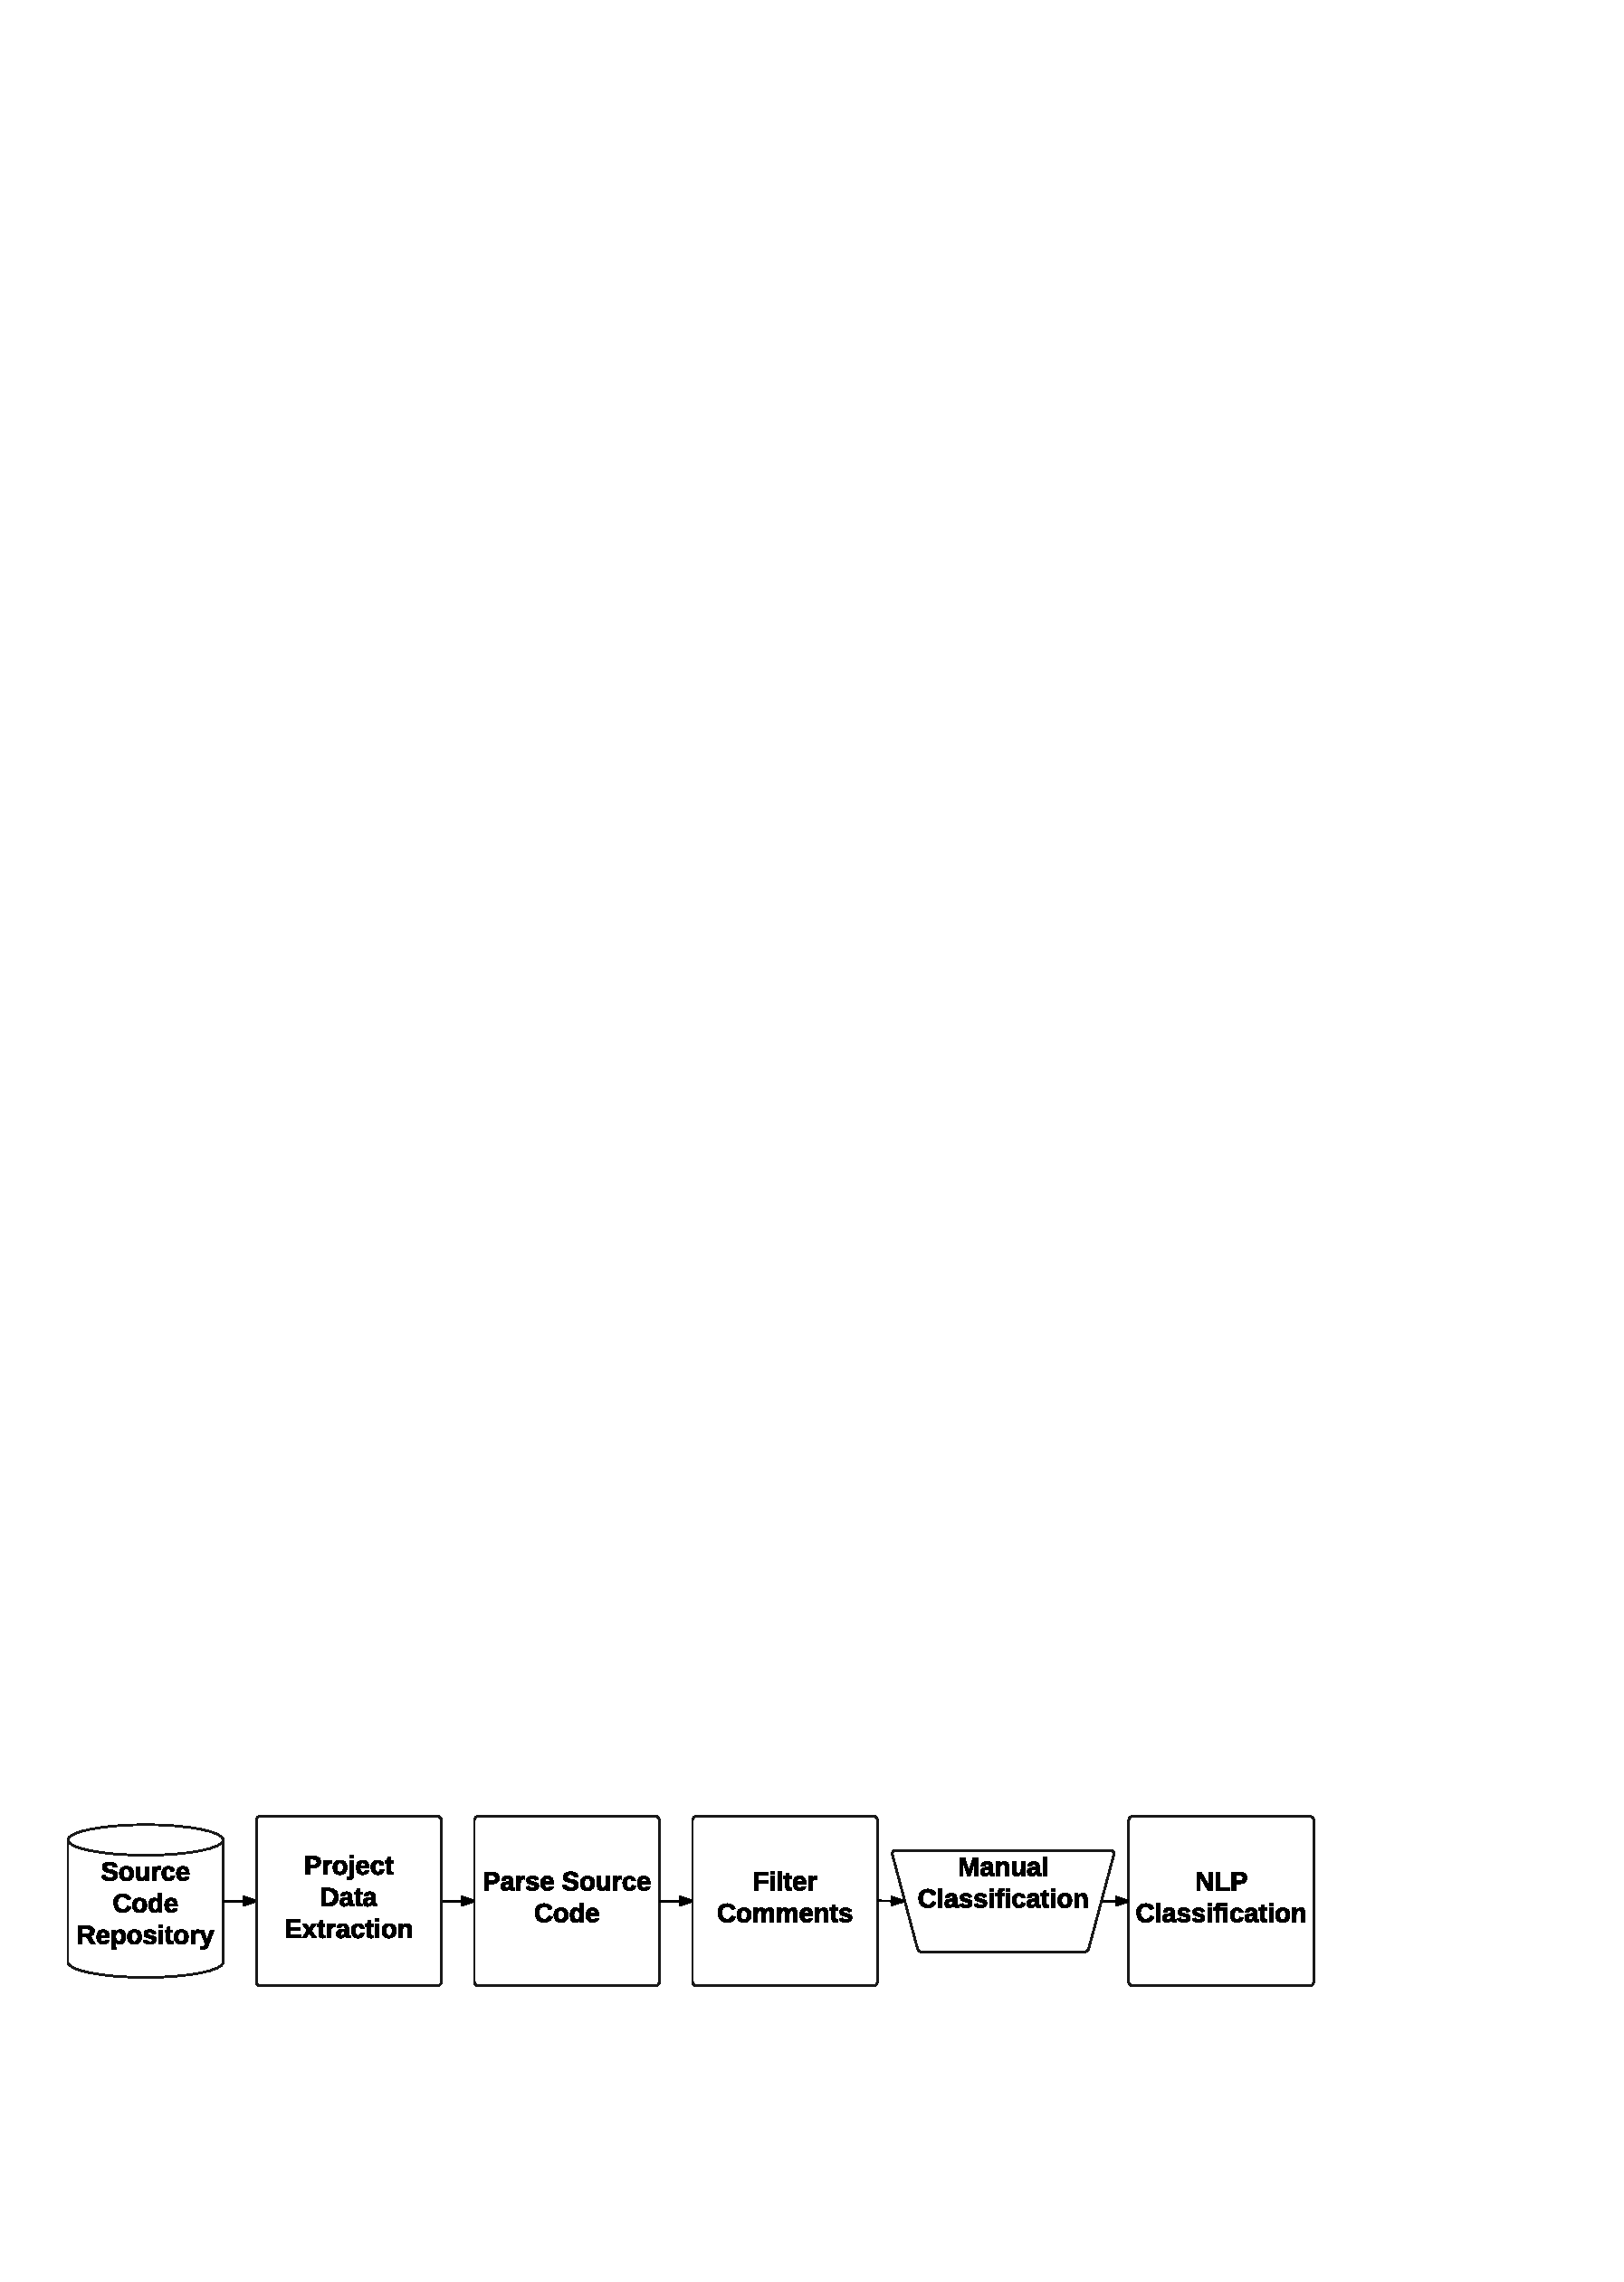
\includegraphics[width=1\textwidth]{figures/approach_reviwed.pdf}
  \caption{Approach Overview}
  \label{fig:approach}
  \vspace{-4mm}
\end{figure*}

The main goal of our study is to automatically identify \SATD through source code comments. To do that, we first extract the comments from ten open source projects. Second, we apply five filtering heuristics to remove comments that are irrelevant for the identification of \SATD  (e.g., license comments, commented source code and Javadoc comments). After that, we manually classify the remaining comments into the different types of \SATD (i.e., design debt, requirement debt, defect debt, documentation debt and test debt). Lastly, we use these comments as training data for the Stanford Classifier and use the trained model to detect \SATD from source code comments. Figure~\ref{fig:approach} shows an overview of our approach, and the following subsections detail each step.

\subsection{Project Data Extraction}
\label{sub:data_extraction}

To perform our study, we need to analyze the source code comments of software projects. Therefore, we extract the source code of ten open source projects: Ant is a build tool written in Java, ArgoUML is an UML modeling tool that includes support for all standard UML 1.4 diagrams, Columba is an email client that has a graphical interface with wizards and internationalization support, EMF is a modeling framework and code generation facility for building tools and other applications, Hibernate is a component providing Object Relational Mapping (ORM) support to applications and other components, JEdit is a text editor written in Java, JFreeChart is a chart library for the Java platform, JMeter is a Java application designed to load test functional behavior and measure performance, JRuby is a pure-Java implementation of the Ruby programming language and SQuirrel SQL is a graphical SQL client written in Java. We selected these projects since they belong to different application domains, are well commented, vary in size, and in the number of contributors. 
    
Table~\ref{tab:project_details} provides details about each of the projects used in our study. The columns of Table~\ref{tab:project_details} present the release used, followed by the number of classes, the total source lines of code (SLOC), the number of contributors, the number of extracted comments, the number of comments analyzed after applying our filtering heuristics, the number of comments that were classified as \SATD, the percentage of these comments that represent design debt, the percentage of \SATD comments classified as requirement debt and finally the percentage of all other types of debt (i.e., defect, documentation and test debt). 

Since there are many different definitions for the SLOC metric we clarify that, in our study, a source line of code contains at least one valid character, which is not a blank space or a source code comment. In addition, we only use the Java files to calculate the SLOC, and to do so, we use the SLOCCount tool~\cite{wheeler2004:home}. 

The number of contributors was extracted from OpenHub, an on-line community and public directory that offers analytics, search services and tools for open source software \cite{Openhub:home}. It is important to note that the number of comments shown for each project does not represent the number of commented lines, but rather the number of Single-line, Block and Javadoc comments. In total, we obtained 259,229 comments, found in 16,249 Java classes. The size of the selected projects varies between 81,307 and 228,191 SLOC, and the number of contributors of these projects ranges from 9 to 326. 

\begin{table*}[thb!]
    \begin{center}
    \caption{Details of Studied Projects}
    \label{tab:project_details}
    \vspace{-5mm}
            \begin{tabular}{l| c c r c || c c c || c c c}
            \toprule
            
            \multirow{5}{*}{\textbf{\thead{Project}}} & \multicolumn{4}{c||}{\textbf{\thead{Project details}}} & \multicolumn{3}{c||}{\textbf{\thead{Comments details}}} & \multicolumn{3}{c}{\textbf{\thead{Technical Debt details}}}

            \\
            \cmidrule{2-11}

            & \textbf{\thead{Release}}  & \textbf{\thead{\# of classes}}   & \textbf{\thead{SLOC}} & \textbf{\thead{\# of \\contributors}}  & \textbf{\thead{\# of \\comments}}   & \textbf{\thead{\# of \\comments \\after filtering}} & \textbf{\thead{\# of \\TD \\comments}} & \textbf{\thead{\% of \\Design \\Debt}} & \textbf{\thead{\% of \\Requirement \\Debt}} & \textbf{\thead{\% of \\Other \\Debts}}\\ 
            \midrule 
            \textbf{Ant}            & 1.7.0    & 1,475 & 115,881 & 74  & 21,587 &   4,137 &    131 &  72.51  & 09.92  & 17.55 \\
            \textbf{ArgoUML}        & 0.34     & 2,609 & 176,839 & 87  & 67,716 &   9,548 &  1,413 &  56.68  & 29.08  & 14.22 \\
            \textbf{Columba}        & 1.4      & 1,711 & 100,200 & 9   & 33,895 &   6,478 &    204 &  61.76  & 21.07  & 17.15 \\
            \textbf{EMF}            & 2.4.1    & 1,458 & 228,191 & 30  & 25,229 &   4,401 &    104 &  75.00  & 15.38  & 09.61 \\
            \textbf{Hibernate}      & 3.3.2 GA & 1,356 & 173,467 & 226 & 11,630 &   2,968 &    472 &  75.21  & 13.55  & 11.22 \\
            \textbf{JEdit}          & 4.2      &   800 &  88,583 & 57  & 16,991 &  10,322 &    256 &  76.56  & 05.46  & 17.96 \\
            \textbf{JFreeChart}     & 1.0.19   & 1,065 & 132,296 & 19  & 23,474 &   4,423 &    209 &  88.03  & 07.17  & 04.78 \\
            \textbf{JMeter}         & 2.10     & 1,181 &  81,307 & 33  & 20,084 &   8,162 &    374 &  84.49  & 05.61  & 09.89 \\
            \textbf{JRuby}          & 1.4.0    & 1,486 & 150,060 & 328 & 11,149 &   4,897 &    622 &  55.14  & 17.68  & 27.17 \\ 
            \textbf{SQuirrel}       & 3.0.3    & 3,108 & 215,234 & 46  & 27,474 &   7,230 &    286 &  73.07  & 17.48  & 09.44 \\ 
            \bottomrule             
        \end{tabular}
    \end{center}
\end{table*}

\subsection{Parse Source Code} 
\label{sub:parse_source_code}

After obtaining the source code of all projects, we extract the comments from the source code. We use JDeodorant \cite{Tsantalis2008CSMR}, an open-source Eclipse plug-in, to parse the source code and extract the code comments. JDeodorant provides detailed information about the source code comments such as: their type (i.e., Block, Single-line, or Javadoc), their location (i.e., the lines where they start and end), and their context (i.e., the method/field/type declaration they belong to).  

Due to these features, we adapted JDeodorant to extract the aforementioned information about source code comments and store it in a relational database to facilitate the processing of the data. 

\subsection{Filter Comments} 
\label{sub:filter_comments}

Source code comments can be used for different purposes in a project, such as giving context, documenting, expressing thoughts, opinions and authorship, and in some cases, disabling source code from the program. Comments are used freely by developers and with limited formalities, if any at all. This informal environment allows developers to bring to light opinions, insights and even confessions (e.g., self-admitted technical debt). 

As shown in prior work, part of these comments can be identified as self-admitted technical debt, but they are not the majority of cases. With that in mind, we develop and apply 5 filtering heuristics to narrow down the comments eliminating the ones that are less likely to be classified as self-admitted technical debt.

To do so, we developed a Java based tool that reads from the database the data obtained by parsing the source code. Next, it executes the filtering heuristics and stores the results back in the database. The retrieved data contains information like the line number that a class/comment starts/ends and the type, considering the Java syntax, of the comment (i.e., Single-line, Block or Javadoc). With this information we process the filtering heuristics as described next.

License comments are not very likely to contain self-admitted technical debt, and are commonly added before the declaration of the class. We create a heuristic that removes comments that are placed before the class declaration. Since we know the line number that the class was declared we can easily check for comments that are placed before that line and remove them. In order to decrease the chances of removing a self-admitted technical debt comment while executing this filter we calibrated this heuristic to not remove comments containing one of task annotations (i.e., ``TODO:'', ``FIXME:'', or ``XXX:'') ~\cite{Storey2008ICSE}. Task annotations are an extended functionality provided by most of the popular Java \textit{IDEs} including Eclipse, InteliJ and NetBeans. When one of these words are used inside a comment the IDE will automatically keep track of the comment creating a centralized list of tasks that can be conveniently accessed later on.

Long comments that are created using multiple \emph{Single-line} comments instead of a \emph{Block} comment can hinder the understanding of the message considering the case that the reader (i.e., human or machine) analyzes each one of these comments independently. To solve that problem, we create a heuristic that searches for consecutive Single-line comments and groups them as one comment.
 
Commented source code is found in the projects due to many different reasons. One of the possibilities is that the code is not currently being used. Other is that, the code is used for debugging purposes only. Based on our analysis, commented source code does not have self-admitted technical debt. Our heuristic removes commented source code using a simple regular expression that captures typical Java code structures.

Automatically generated comments by the IDE are filtered out as well. These comments are inserted as part of code snippets used to generate constructors, methods and try catch blocks, and have a fixed format (i.e., ``Auto-generated constructor stub'', ``Auto-generated method stub'', and ``Auto-generated catch block''). Therefore our heuristic searches for these automatically generated comments and removes them. 

Javadoc comments rarely mention self-admitted technical debt. For the Javadoc comments that do mention self-admitted technical debt, we notice that they usually contain one of the task annotations (i.e., ``TODO:'', ``FIXME:'', or ``XXX:''). Therefore, our heuristic removes all comments of the type Javadoc unless they contain at least one of the task annotations  To do so, we create a simple regular expression that searches for the task annotations before removing the comment.  

The steps mentioned above significantly reduced the number of comments in our dataset and helped us focus on the most applicable and insightful comments. For example, in the Ant project, applying the above steps helped to reduce the number of comments from 21,587 to 4,137 meaning a reduction of 80.83\% in the number of comments to be manually analyzed. Using the filtering heuristics we were able to remove from 39.25\% to 85.89\% of all comments. Table \ref{tab:project_details} provides the number of comments kept after the filtering heuristics for each project.

\subsection{Manual Classification}
\label{sub:manual_classification}

Our goal is to inspect each comment and attribute to it the suitable technical debt classification. Since there are many comments, we developed a Java based tool that shows one comment at a time and gives a list of possible classifications that can be manually assigned to the comment. The list of possible classifications is based on previous work by Alves \textit{et al.}~\cite{Alves2014MTD}. In their work, an ontology on technical debt terms was proposed, and they identified the following types of technical debt across the researched literature: architecture, build, code, defect, design, documentation, infrastructure, people, process, requirement, service, test automation and test debt. During the classification process we notice that not all types of debt mentioned by Alves \emph{et al.}~\cite{Alves2014MTD} could be found in code comments. However, we were able to identify the following types of debt in the source comments: design debt, defect debt, documentation debt, requirement debt and test debt. 

In our previous work ~\cite{Maldonado2015MTD} we manually classified 33,093 comments, and in the current study we manually classified an additional 29,473 comments, which means that we extended our classified comments dataset by 89.06\%. In total, we manually classified 62,566 comments into the five different types of self-admitted technical debt mentioned above. The classification process took approximately 185 hours in total, and was performed by the first author of the paper. It is important to note here that this manual classification step does not need to be repeated in order to apply our approach, since our dataset is publicly available, and thus it can used as is, or even extended with new classified comments. 

  
Below, we provide definitions for design and requirement \SATD, and some indicative comments to help the reader understand the different types of self-admitted technical debt comments.

\vspace{1mm}
\noindent\textbf{Self-admitted design debt:} These comments indicate that there is a problem with the design of the code. They can be comments about misplaced code, lack of abstraction, long methods, poor implementation, workarounds, or temporary solutions. Usually these kinds of issues are resolved through refactoring (i.e., restructuring of \emph{existing} code), or by re-implementing \emph{existing} code to make it faster, more secure, more stable and so forth. Let us consider the following comments:

\vspace{1mm}
    \begin{displayquote}
        \textit{``TODO: - This method is too complex, lets break it up''} - [from ArgoUml]
    \end{displayquote}
    \vspace{1mm}
    \begin{displayquote}
     \textit{``/* TODO: really should be a separate class */''} - [from ArgoUml]
    \end{displayquote}
\vspace{1mm}

These comments are clear examples of what we consider as self-admitted \emph{design debt}. In the above comments, the developers state what needs to be done in order to improve the current design of the code, and
the payback of this kind of design debt can be achieved through refactoring.
Although the above comments are easy to understand, during our study we came across more challenging comments that expressed design problems in an indirect way. For example: 

\vspace{1mm}
    \begin{displayquote}
        \textit{``// I hate this so much even before I start writing it. // Re-initialising a global in a place where no-one will see it just // feels wrong.  Oh well, here goes.''} - [from ArgoUml]
    \end{displayquote}
    \vspace{1mm}
    \begin{displayquote}
        \textit{``//quick \& dirty, to make nested mapped p-sets work:''} - [from Apache Ant]
    \end{displayquote}
\vspace{1mm}

In the above example comments the authors are certain to be implementing code that does not represent the best solution. Intuitively, we know that kind of implementation will degrade the design of the code and should be avoided. 

\vspace{1mm}
    \begin{displayquote}
        \textit{``// probably not the best choice, but it solves the problem of // relative paths in CLASSPATH''} - [from Apache Ant]
    \end{displayquote}
    \vspace{1mm}
    \begin{displayquote}   
        \textit{``//I can't get my head around this; is encoding treatment needed here?''} - [from Apache Ant]
    \end{displayquote}
\vspace{1mm}

The above comments expressed doubt and uncertainty when implementing the code and were considered as self-admitted design debt as well.
The payback of the design debt expressed in the last four example comments can be probably achieved through the re-implementation of the currently existing solution.

\vspace{1mm}
\noindent\textbf{Self-admitted requirement debt:} These comments convey the opinion of a developer supporting that the implementation of a requirement is not complete.  In general, requirement debt comments express
that there is still \emph{missing} code that needs to be added in order to complete a \emph{partially} implemented requirement, as it can be observed in the following comments:

\vspace{1mm}
    \begin{displayquote}
        \textit{``/TODO no methods yet for getClassname''} - [from Apache Ant]
    \end{displayquote}
    \vspace{1mm}
    \begin{displayquote}
        \textit{``//TODO no method for newInstance using a reverse-classloader''} - [from Apache Ant]
    \end{displayquote}
    \vspace{1mm}
    \begin{displayquote}
        \textit{``TODO: The copy function is not yet * completely implemented - so we will  * have some exceptions here and there.*/''} - [from ArgoUml]  
    \end{displayquote}
    \vspace{1mm}
    \begin{displayquote}
        \textit{``TODO: This dialect is not yet complete. Need to provide implementations wherever \textit{Not yet implemented} appears''} - [from SQuirrel]  
    \end{displayquote}
    \vspace{1mm}
\vspace{1mm}  

To mitigate the risk of creating a dataset that is biased, we extracted a statistically significant sample of our dataset and asked another student to classify it. To prepare the student for the task we gave a 1-hour tutorial about the different kinds of \SATD, and walked the student through a couple of examples of each different type of \SATD comment. The statistically significant sample was created based on the total number of comments (62,566) with a confidence level of 99\% and a confidence interval of 5\%. Resulting in a stratified sample of 659 comments. We composed the stratified sample according to the percentage of each classification found in the original dataset. Therefore, the stratified sample was composed of: 92\% of without \SATD comments (609 comments), 4\% of design debt comments (29 comments), 2\% of requirements debt comments (5 comments), 0.75\% test debt (2 comments) and 0.15\% of documentation debt (1 comment). Lastly, we evaluate the level of agreement between both reviewers of the stratified sample by calculating Cohen's kappa coefficient ~\cite{cohen1960coefficient}. Cohen's Kappa coefficient has been commonly used to evaluate inter-rater agreement level for categorical scales, and provides the proportion of agreement corrected for chance. The resulting coefficient is scaled to range between -1 and +1, where negative value means poorer than chance agreement, zero indicates exactly chance agreement, and positive value indicates better than chance agreement ~\cite{fleiss1973equivalence}. The closer the value is to +1, the better. In our work, the level of agreement measured between the reviewers was of +0.81.

We also measured the level of agreement of design and requirement \SATD individually. This is important because the stratified sample possesses much more without \SATD comments than the other types of debt, and therefore, the coefficient reported above could indicate that the reviewers are agreeing on what is not \SATD instead of agreeing on a particular type of debt. However, we achieved a level of agreement of +0.75 for design \SATD, and +0.85 for requirement \SATD. According to Fleiss~\cite{Fleiss1981measurement} values larger than 0.75 are characterized as excellent.

\subsection{NLP Classification}
\label{sub:run_the_nlp_classifier}

Our next step is to use the classified \SATD comments as a training dataset for the  Stanford Classifier, which is a Java implementation of a max entropy classifier}{R2-11}~\cite{Manning2014ACL}. A max entropy classifier}{R2-11}, in general, takes as input a number of data items along with a classification for each data item, and automatically generates \textit{features} (i.e., words) from each \textit{datum}, which are associated with positive or negative numeric \textit{votes} for each class. The weights of the features are learned automatically based on the manually classified training data items (supervised learning). The  Stanford Classifier}{R2-11} builds a \textit{maximum entropy model}, which is equivalent to a multi-class regression model, and it is trained to maximize the conditional likelihood of the classes taking into account feature dependences when calculating the feature weights.

After the training phase, the  max entropy classifier can take as input a test dataset that will be classified according to the model built during the training phase. The output for each data item of the test dataset is the classification, along with the features contributing positively or negatively in this classification.

In our case, the training dataset is composed of source code comments and their corresponding manual classification.
According to our findings in previous work~\cite{Maldonado2015MTD}, the two most common types of \SATD are design and requirement debt (defect, test, and documentation debt together represent less that 10\% of all \SATD comments).
Therefore, we train the Stanford Classifier on the dataset containing only these two specific types of \SATD comments.

In order to avoid having repeated features differing only in letter case (e.g., ``Hack'', ``hack'', ``HACK''), or in preceding/succeeding punctuation characters (e.g., ``\textbf{,}hack'', ``hack\textbf{,}''), we preprocess the training and test datasets to clean up the original comments written by the developers. More specifically, we remove the character structures that are used in the Java language syntax to indicate comments (i.e., `//' or `/*' and `*/'), the punctuation characters, and any excess whitespace characters (e.g., ` ', `\textbackslash t', `\textbackslash n'), and finally we convert all comments to lowercase.  However, we decided to not remove exclamation and interrogation points. These specific punctuation was very useful during the identification of \SATD comments, and provides insightful information about the meaning of the features.                                                                                                                                                                                                                                                                                                                                                                                                                                                                                                                                                                                                                                                                                                                                                                                                                      